\documentclass[angelino.tex]{subfiles} 
\begin{document}

We attack the general problem of accelerating MCMC algorithms
by using speculative execution to parallelize them.
In the previous chapter, our survey of MCMC methods included
this approach, sometimes called \emph{prefetching}.
An effective prefetching implementation must overcome several challenges,
such as correctness.
For example, for the results of prefetching to exactly equal those of a
serial execution, care is required in the treatment of pseudo-randomness
(\ie each node's source of randomness must produce the same results
as it would in a serial execution); slapdash treatment risks introducing biases.
%
But the key challenge for prefetching is performance.
A na\"{i}ve scheduling scheme always requires~${\approx 2^J}$ parallel cores to 
achieve a speedup of~$J$.
As we saw, this speedup can be improved by leveraging information about the
average proposal acceptance rate~\citep{strid-2010-prefetching}.
%
In particular, if most proposals are rejected, a prefetching implementation
can improve its speedup by prefetching more heavily along the reject path.
%
Although in practice the optimal acceptance rate is less than 
0.5~\citep{roberts-1997-accept}, extremely small acceptance rates,
which lead to good speedup, are accompanied by less effective mixing.
If the acceptance rate is set to something like~0.234,
speedup is still at most logarithmic.

In this chapter, we propose \emph{predictive prefetching}, a new scheduling
approach that uses local information to improve speedup relative to other 
prefetching schemes.
%
First, we provide a general mathematical framework that allows us to identify a
broad class of MCMC algorithms that can benefit from prefetching.
%
Second, we carefully reason about Metropolis--Hastings in a way that maps
naturally to prefetching schemes.
%
Next, we describe our predictive prefetching scheme, where we adaptively adjust 
speculation based not only on the local average proposal acceptance rate --
which changes as evaluation progresses --
but also on the actual random deviate used at each state.
%
In particular, we describe how we make use of any available fast approximations
to the transition operator.
%
Though these approximations are not required, when they are available or
learnable, we leverage them to make better scheduling decisions.
%
For the special case of large-scale Bayesian inference,
we develop a series of increasingly expensive but more accurate approximations.
%
These decisions are further improved by modeling the error of these
approximations, and thus the uncertainty of the scheduling decisions.
%
Performance depends critically on how we model the approximations,
and a key insight is in our error model for this setting;
much smaller error, and therefore more precise predictions,
are obtained by modeling the error of the \emph{difference} between two proposal 
evaluations, rather than evaluating the errors of the proposals separately.
%
Finally, we provide a theoretical analysis of speedup due to predictive
prefetching as a function of predictor accuracy and the number parallel cores.
%
In the next chapter, we describe the details of our system design and
implementation, and in the following chapter, we present our actual
empirical results.

\section{Mathematical framework}
\label{sec:mathematical-framework}

Consider a transition operator~${T(x \to x')}$ which has~$\pi$ as its stationary 
distribution on state space~$\X$.
Simulation of such an operator typically proceeds using an `external' source of 
pseudo-random numbers that can, without loss of generality, be assumed to be
drawn uniformly on the unit hypercube, denoted as~$\mcU$.
The transition operator is then a deterministic function from the product space 
of~$\mcU$ and~$\X$ back to~$\X$, \ie~${T:\X\times\mcU\to\X}$.
Most practical transition operators -- Metropolis--Hastings, slice sampling,
{\it etc.} -- are actually compositions of two such functions, however.
The first function produces a countable set of candidate points in~$\X$, here denoted~${Q:\X\times\mcU_Q\to\mcP(\X)}$, where~$\mcP(\X)$ is the power set of~$\X$.  The second function~${R:\mcP(\X)\times\mcU_R\to\X}$ then chooses one of the candidates for the next state in the Markov chain.  Here we have used~$\mcU_Q$ and~$\mcU_R$ to indicate the disjoint subspaces of~$\mcU$ relevant to each part of the operator.
In this setup, the basic Metropolis--Hastings algorithm uses~$Q(\cdot)$
to produce a tuple of the current point and a proposed point, while
multiple-try MH~\citep{liu:2000-multiple-try} and
delayed-rejection MH~\citep{tierney:1999-adaptive,green:2001-delayed-rejection},
each create a larger candidate set that includes the current point.
In the exponential-shrinkage variant of slice sampling~\citep{neal:2003-slice},
the function~$Q(\cdot)$ produces an infinite sequence of candidates that
converges to, but does not include, the current point.

This setup is a somewhat more elaborate treatment than usual, but this is intended to serve two purposes: 1)~make it clear that there is a separation between generating a set of possible candidates via~$Q(\cdot)$ and selecting among them with~$R(\cdot)$, and 2)~highlight that both of these functions are deterministic functions, given the pseudo-random variates.
Others have observed this latter point and used it to construct alternative 
approaches to MCMC~\citep{propp-wilson-1996a, neal:2012a-permutation}.

We separately consider~$Q(\cdot)$ and~$R(\cdot)$, because it is generally the case that~$Q(\cdot)$ is inexpensive to evaluate and does not require computation of the target density~$\pi(x)$, while~$R(\cdot)$ must compare the target density at the candidate locations and so represents the bulk of the computational burden.  Prefetching MCMC observes that, since~$Q(\cdot)$ is cheap and the pseudo-random variates can be produced in any order, the tree of possible future states of the Markov chain can be constructed before any of the~$R(\cdot)$ functions are evaluated, as in Figure~\ref{tree} and reproduced here for convenience in Figure~\ref{tree-copy}.  The sequence of~$R(\cdot)$ evaluations simply chooses a path down this tree.  
We parallelize execution by speculatively choosing to evaluate~$R(\{x_i\}, u)$ for some parts of the tree that have not yet been reached.  If one or more nodes in this subtree are eventually reached, then we achieve a speedup.

\begin{figure}[t!]
  \centering%
  \resizebox{\columnwidth}{!}{%
    \def\radius {5mm}
    \tikzstyle{state}=[circle, thick, minimum size=\radius, font=\footnotesize]
    \begin{tikzpicture}[->,>=stealth',level/.style={sibling distance = 5cm/#1, level distance = 1.5cm}]
      \draw [white,-] (-6cm,-0.75cm) -- (6cm,-0.75cm);
   %   \draw [gray,-] (-6cm,-2.25cm) -- (6cm,-2.25cm);
   %   \draw [gray,-] (-6cm,-3.75cm) -- (6cm,-3.75cm);
      \node [state] {$x^t$}
      child{ node [state] {$x^{t+1}_\bits{0}$}
        child{ node [state] {$x^{t+2}_{\bits{00}}$}
          child{ node [state] {$x^{t+3}_{\bits{000}}$}}
          child{ node [state] {$x^{t+3}_{\bits{001}}$}}
        }
        child{ node [state] {$x^{t+2}_{\bits{01}}$}
          child{ node [state] {$x^{t+3}_{\bits{010}}$}}
          child{ node [state] {$x^{t+3}_{\bits{011}}$}}
        }
      }
      child{ node [state] {$x^{t+1}_1$}
        child{ node [state] {$x^{t+2}_{\bits{10}}$}
          child{ node [state] {$x^{t+3}_{\bits{100}}$}}
          child{ node [state] {$x^{t+3}_{\bits{101}}$}}
        }
        child{ node [state] {$x^{t+2}_{\bits{11}}$}
          child{ node [state] {$x^{t+3}_{\bits{110}}$}}
          child{ node [state] {$x^{t+3}_{\bits{111}}$}}
        }
      }
      ;
      %\node [state] at (5.5cm, 0) {$u^{t}$};
      %\node [state] at (5.5cm, -1.5) {$u^{t+1}$};
      %\node [state] at (5.5cm, -3) {$u^{t+2}$};
      %\node [state] at (5.5cm, -4.5) {$u^{t+3}$};
    \end{tikzpicture}
  }
  \caption{Metropolis--Hastings conceptualized as a binary tree.
  Each level of the tree represents an iteration, where branching to the
  right/left indicates that the proposal is accepted/rejected.
  Each subscript is a sequence of \bits{0}'s and \bits{1}s
  corresponding to the history of rejected and accepted proposals
  with respect to the root.  
  %The random variates (on right) are shared across the layer.}
  (Reproduced from Figure~\ref{tree}.)
  }
  \label{tree-copy}
\end{figure}

For clarity, in the remainder of this thesis we focus on the
straightforward random-walk Metropolis--Hastings operator;
we depict our view of its simulation in Algorithm~\ref{mh-decomposed}.
In this special case,~$Q(\cdot)$ produces a tuple of the current point and a 
proposal.
The function~${R:\X\times\X\times(0,1)\to\X}$ takes these two points, along with a uniform random variate in~$(0,1)$, and selects one of the two inputs via:
\begin{align}
R(x,x',u) &= \begin{cases}
 x' & \text{if } u\dfrac{q(x' \given x)}{q(x \given x')} < \dfrac{\pi(x')}{\pi(x)}\\
 x & \text{otherwise}
 \end{cases}\,,
 \label{eqn:mh-threshold}
\end{align}
where~$q(\cdot\given\cdot)$ is the proposal density corresponding to~$Q(\cdot)$.  We write the acceptance ratio in this somewhat unusual fashion to highlight the fact that the left-hand side of the inequality does not require evaluation of the target density and is easy to precompute.

\begin{algorithm}[t]
\caption{Our view of Metropolis--Hastings.}
\label{mh-decomposed}
\begin{algorithmic}
\State \textbf{Input:} Initial state~$x^0$, number of iterations~$T$, target~$\pi(x)$, proposal~$q(x' \given x)$
\State \textbf{Output:} Samples $x^1, \dots, x^T$
\For {$t$ in $0, \dots, T-1$}
\vspace{1mm}
\State $\uu_Q^t = \{u_{Q,i}^t \sim \Unif(0, 1)\}$
	\Comment{Pseudo-random numbers consumed by $Q(\cdot)$}
\vspace{1mm}
\State $u_R^t \sim \Unif(0, 1)$
	\Comment{Pseudo-random number for $R(\cdot)$}
\vspace{1mm}
\State $(x^t, x') \gets Q(x^t, \mathbf{u}_Q^t) = (x^t, x' \sim q(x' \given x))$
	\Comment{Produce two candidates}
\vspace{1mm}
\State $x^{t+1} \gets R(x^t, x', u_R^t) = 
\begin{cases}
x' \quad \text{if}~u_R^t \dfrac{q(x' \given x^t)}{q(x^t \given x')} < \dfrac{\pi(x')}{\pi(x^t)} \\
x^t \quad \text{otherwise}
\end{cases}$
\Comment{Select next state}
\EndFor
\end{algorithmic}
\end{algorithm}

\section{Metropolis--Hastings simulation}

In this section, we reason about Metropolis--Hastings simulation through the
lens of the binary state tree.
This enables us to coherently reason about prefetching schemes as well as
motivate and describe our approach in the next section.
%
First, we develop some notation that gives us a language for talking about
the MH tree.
This notation will also map to the data structures and routines
used in our system design, described in the next chapter.
%
Now, recall that prefetching schemes use parallel cores to precompute the target
density at states that might be considered during simulation.
Thus, we next use the tree to identify where computation occurs with respect to
a particular simulation and then discuss the use of pseudo-randomness with
respect to the tree.
Finally, we introduce a new binary tree, the \emph{jobtree}, that simplifies how to reason about
computation during MH simulation; this will help us cleanly describe our
approach in the next section and will form the central data structure of our
system in the next chapter.

\subsection{Bit string notation}
\label{sec:bit-strings}

We use small Greek letters ($\alpha$, $\beta$) for elements of $\{0,1\}^*$.
Let $\emptystr$ be the empty string.
Given a bit string $\alpha$, let $\truncbits{\alpha}$ equal $\alpha$
with all trailing $\bits{0}$ bits removed.
%and let $\|\alpha\|$ be the length of $\alpha$.
%Define $\xtruncbits{\alpha}$ as follows:
%%
%\[ \xtruncbits{\alpha} = \begin{cases}
%    \truncbits{\alpha} & \text{if $\truncbits{\alpha} \neq
%    \emptystr$,} \\
%    \bits{0} & \text{if $\truncbits{\alpha} = \emptystr$.}
%   \end{cases} \]
%%
%That is, $\xtruncbits{\alpha}$ normally equals $\truncbits{\alpha}$,
%except that $\xtruncbits{\bits{0}^i} = \bits{0}$.
Define $\bitsflip{\alpha}$ as $\alpha$ with the last bit flipped, as
follows:
%
\[ \bitsflip{\alpha} = \begin{cases}
   \bits{1} & \text{if $\alpha = \emptystr$,} \\
   \beta\bits{1} & \text{if $\alpha = \beta\bits{0}$,} \\
   \beta\bits{0} & \text{if $\alpha = \beta\bits{1}$.}
   \end{cases} \]

\subsection{Mapping states to bit strings}

Recall from Figure~\ref{tree-copy} that we can conceptualize
Metropolis--Hastings as a binary tree: given the current state,
the possible sequences of future states result from accepting or rejecting
a proposal at each iteration.
We reproduce this tree in Figure~\ref{tree-colored}, this time with different
colors to highlight sequences of possible Markov chain states that are
identical, due to sequences of rejected proposals.
Each node is labeled with a distinct subscript, mapping each possible state
to a bit string that records the history of the chain, as we describe below.

\begin{figure}[t!]
  \centering%
  \resizebox{\columnwidth}{!}{%
    \def\radius {8mm}
    \tikzstyle{state}=[circle, thick, minimum size=\radius, font=\footnotesize]
    \tikzstyle{s1}=[circle, thick, draw, fill=CornflowerBlue, minimum size=\radius, inner sep=0pt, font=\footnotesize]
    \tikzstyle{s2}=[circle, thick, draw, fill=LightBlue, minimum size=\radius, inner sep=0pt, font=\footnotesize]
    \tikzstyle{s3}=[circle, thick, draw, fill=LightSteelBlue, minimum size=\radius, inner sep=0pt, font=\footnotesize]
    \tikzstyle{s4}=[circle, thick, draw, fill=LightGrey, minimum size=\radius, inner sep=0pt, font=\footnotesize]
    \begin{tikzpicture}[->,>=stealth',level/.style={sibling distance = 5cm/#1, level distance = 1.5cm}]
      \draw [white,-] (-6cm,-0.75cm) -- (6cm,-0.75cm);
    %  \draw [gray,-] (-6cm,-2.25cm) -- (6cm,-2.25cm);
    %  \draw [gray,-] (-6cm,-3.75cm) -- (6cm,-3.75cm);
      \node [s1] {$x^t_\emptystr$}
      child{ node [s1] {$x^{t+1}_\bits{0}$}
        child{ node [s1] {$x^{t+2}_{\bits{00}}$}
          child{ node [s1] {$x^{t+3}_{\bits{000}}$}}
          child{ node [state] {$x^{t+3}_{\bits{001}}$}}
        }
        child{ node [s2] {$x^{t+2}_{\bits{01}}$}
          child{ node [s2] {$x^{t+3}_{\bits{010}}$}}
          child{ node [state] {$x^{t+3}_{\bits{011}}$}}
        }
      }
      child{ node [s3] {$x^{t+1}_1$}
        child{ node [s3] {$x^{t+2}_{\bits{10}}$}
          child{ node [s3] {$x^{t+3}_{\bits{100}}$}}
          child{ node [state] {$x^{t+3}_{\bits{101}}$}}
        }
        child{ node [s4] {$x^{t+2}_{\bits{11}}$}
          child{ node [s4] {$x^{t+3}_{\bits{110}}$}}
          child{ node [state] {$x^{t+3}_{\bits{111}}$}}
        }
      }
      ;
%      \node [state] at (5.5cm, 0) {$\uu^{t}$};
%      \node [state] at (5.5cm, -1.5) {$\uu^{t+1}$};
%      \node [state] at (5.5cm, -3) {$\uu^{t+2}$};
%      \node [state] at (5.5cm, -4.5) {$\uu^{t+3}$};
    \end{tikzpicture}
  }
  \caption{Metropolis--Hastings conceptualized as a binary tree.
  Each level of the tree represents an iteration, where branching to the
  right/left indicates that the proposal is accepted/rejected.
  Each subscript is a sequence of \bits{0}'s and \bits{1}'s
  corresponding to the history of rejected and accepted proposals
  with respect to the current state~$x^t$ at the root.
  Nodes of the same color correspond to sequences of states that are equal,
  which happens when proposals are rejected.
  For example, the nodes along the left-most branch are all equal to the root
  and correspond to a sequence of three rejected proposals.
  The four uncolored nodes at the bottom of the tree represent the possible 
  proposals at iteration~$t+3$ and are distinct.
  } 
  \label{tree-colored}
\end{figure}

Without loss of generality, call the current state~$x^0$.
Let iteration~$t$ simulate the transition from a state~$x^t$ to the next 
state~$x^{t+1}$, as in our descriptions of Metropolis--Hastings in
Algorithms~\ref{mh} and~\ref{mh-decomposed}.
For all~$t \ge 0$, define a mapping~$\rho(x^t) \equiv \rho^t$
that identifies with each possible state~$x^t$ a bit string~$\rho^t$,
relative to the current state~$x^0$, as follows:
%
\[ \rho(x^t) = \begin{cases}
   \emptystr & \text{if $t=0$,} \\
   \rho^{t-1}\bits{1} & \text{if $t>0$ and proposal at iteration $t$ is accepted,}  \\
   \rho^{t-1}\bits{0} & \text{otherwise, in which case the proposal is rejected and $x^t = x^{t-1}$.}
  \end{cases} \]
%
In other words, the current state~$x^0$ is mapped to~$\emptystr$ and
otherwise,~$x^t$ is mapped to a sequence of $\bits{0}$'s and $\bits{1}$'s
corresponding to its history of rejected and accepted proposals, respectively.
The length of~$\rho^t$ is~$t$ and $\rho^t$ is a prefix of
$\rho^T$ for all $T \geq t$.
%Define $\Theta$ as the infinite-length limit of $\Theta^i$.
Note that an inverse mapping from bit strings to states, 
\ie~$\rho^{-1}(\rho^t) = x^t$,
must satisfy~$\rho^{-1}(\alpha) = \rho^{-1}(\truncbits{\alpha})$.
This corresponds to the fact that sequences of rejected proposals yield
sequences of Markov chain states equal to either the last accepted proposal
or the initial state, if no such proposal exists.

%\noindent If $\alpha \neq \rho_{\|\alpha\|}$, then it does not
%matter what $\lambda(\alpha)$ is.

%The perturbation step that takes us from $\theta(\alpha)$
%to $\theta(\alpha\bits{1})$ does not depend on how good the current
%point is, i.e., we do not need to know $\Pr(\theta(\alpha) \mid x)$ in order to
%calculate the proposal $\theta(\alpha\bits{1})$.
%For our purposes, if the length of $\alpha$ is $i$,
%the $i$-th perturbation, $\Delta_i = \theta(\alpha\bits{1}) - \theta(\alpha)$, 
%is the $i$-th draw from a so-called jumping distribution that does not 
%depend on $\Pr(\theta(\alpha) \mid x)$ or even $\theta(\alpha)$. 
%For example, if the parameter sets correspond to real vectors of length $n$,
%$\Delta_i$ could be drawn from a fixed $n$-dimensional normal distribution.
%This is why, given $\theta_0$ and a source of randomness, 
%we can generate the whole tree of all possible values of the $\theta^i$'s 
%before we calculate any of their probabilities.
%Note that $\Delta_i$ could depend on the history of the chain, as would be the
%case with adaptive MH. %or something like simulated annealing.

\subsection{Computation with respect to a simulation path}

\begin{figure}[t!]
  \centering%
  \resizebox{\columnwidth}{!}{%
    \def\radius {8mm}
    \tikzstyle{state}=[circle, thick, minimum size=\radius, font=\footnotesize]
    \tikzstyle{path}=[circle, thick, fill=LightBlue, inner sep=0pt, minimum size=\radius, font=\footnotesize, draw]
    \tikzstyle{compute}=[circle, thick, fill=CornflowerBlue, inner sep=0pt, minimum size=\radius, font=\footnotesize, draw]
    \begin{tikzpicture}[->,>=stealth',level/.style={sibling distance = 5cm/#1, level distance = 1.5cm}]
      \draw [white,-] (-6cm,-0.75cm) -- (6cm,-0.75cm);
   %   \draw [gray,-] (-6cm,-2.25cm) -- (6cm,-2.25cm);
   %   \draw [gray,-] (-6cm,-3.75cm) -- (6cm,-3.75cm);
      \node [compute] (root) {$x^t_\emptystr$}
      child{ node [state] {$x^{t+1}_\bits{0}$}
        child{ node [state] {$x^{t+2}_\bits{00}$}
          child{ node [state] {$x^{t+3}_\bits{000}$}}
          child{ node [state] {$x^{t+3}_\bits{001}$}}
        }
        child{ node [state] {$x^{t+2}_\bits{01}$}
          child{ node [state] {$x^{t+3}_\bits{010}$}}
          child{ node [state] {$x^{t+3}_\bits{011}$}}
        }
      }
      child{ node [compute] {$x^{t+1}_\bits{1}$}
        child{ node [path] {$x^{t+2}_\bits{10}$}
          child{ node [path] {$x^{t+3}_\bits{100}$}}
          child{ node [compute] {$x^{t+3}_\bits{101}$}}
        }
        child{ node [compute] {$x^{t+2}_\bits{11}$}
          child{ node [state] {$x^{t+3}_\bits{110}$}}
          child{ node [state] {$x^{t+3}_\bits{111}$}}
        }
      }
      ;
   %   \node [state] at (5.5cm, 0) {$\uu^{t}$};
   %   \node [state] at (5.5cm, -1.5) {$\uu^{t+1}$};
   %   \node [state] at (5.5cm, -3) {$\uu^{t+2}$};
   %   \node [state] at (5.5cm, -4.5) {$\uu^{t+3}$};
      \draw [->, ultra thick, Dandelion] (root) to (root-2);
      \draw [->, ultra thick, Dandelion] (root-2) to (root-2-1);
      \draw [->, ultra thick, Dandelion] (root-2-1) to (root-2-1-1);
    \end{tikzpicture}
  }
  \caption{Schematic of a Metropolis--Hastings simulation superimposed on the
  binary tree of all possible states. 
  As in Figure~\ref{tree-copy}, each level of the tree represents an iteration,
  where branching to the right/left 
  indicates that the proposal is accepted/rejected.
  The simulation path (thick arrows) starts at the root~$x^t$
  and connects the output states: $x_1^{t+1}, x_{10}^{t+2}, x_{100}^{t+3}$.
  In this example, the first proposal is accepted and
  the next two proposals are rejected.  
  The dark filled circles indicate states where the target density
  is evaluated during simulation.
  Those that are not on the simulation path correspond to rejected proposals.
  Their siblings are pale filled circles on the simulation path;
  since each of the corresponding states is a copy of its parent,
  its target density does not need to be reevaluated during the subsequent
  comparison to the next proposal.}
  \label{tree-chain}
\end{figure}

Figure~\ref{tree-chain} depicts one instance of a Metropolis--Hastings
simulation superimposed on the binary tree of all possible states.
As before, left and right children correspond to the state
after a proposal has been rejected or accepted, respectively.
Given the current state at the root, the states of the simulated Markov chain
correspond to a single connected path through the tree.
We call this the \emph{simulation path}.

Each iteration simulates one MH transition and involves evaluating the target
density at a new proposal.
A node corresponding to a rejected proposal is \emph{not} directly on the
simulation path, but its left sibling and parent as well as other ancestors are
all on the simulation path.
The state at the left sibling is equal to the state at the parent.
Thus, the MH algorithm involves computations at and only at three kinds of
nodes: the root, nodes on the simulation path that are right children 
(accepted proposals) and the right siblings of nodes on the simulation path that
are left children (rejected proposals).

\subsection{Using pseudo-randomness}
\label{sec:using-randomness}

%In Section~\label{sec:mathematical-framework}, we described a broad class
%of transition operators as functions from the product space 
%of~$\X$ and~$\mcU$ back to~$\X$, \ie~${T:\X\times\mcU\to\X}$.
%Simulating one such transition consumes multiple numbers from a pseudo-random
%stream that, without loss of generality, we think of together as
%a uniform random draw from~$\mcU$, the unit hypercube.
%In our description of Metropolis--Hastings in Algorithm~\ref{mh-decomposed},
%iteration~$t$ consumes at least one random variate~$\uu_Q^t$ to generate the
%proposal and exactly one random variate~$u_R^t$.
%Denote the uniform variates consumed at iteration~$t$ as~$\uu^t$.

For a particular transition operator~$T(x \rightarrow x')$ as described in 
Section~\ref{sec:mathematical-framework}, the number of random variates required
to simulate one transition in general depends on the starting state~$x$.
%
For example, in Metropolis--Hastings as described in
Algorithm~\ref{mh-decomposed}, iteration~$t$ consumes
at least one random variate~$\uu_Q^t$ to generate the proposal
plus exactly one random variate~$u_R^t$ to select the next state. 
%
The MH proposal step can easily consume a non-constant number of random
variates, \eg if the proposal is generated via rejection sampling,
as is common when dealing with truncated distributions.

This subtle point matters when thinking about prefetching schemes
as it implies that the consumption of a pseudo-random stream during
Markov chain simulation depends on the history of the chain.
%
With respect to the MH tree as illustrated in Figure~\ref{tree},
this means that a pseudo-random stream may be consumed at different rates,
depending on what simulation path is taken on the tree.
%
From our reading of prior work on prefetching, it is not clear to us whether
this issue has been addressed or ignored;
\eg \citet{strid-2010-prefetching} casually refers to the handling of
pseudo-random numbers in prefetching schemes as ``an implementation issue.''

In our use of prefetching, given an initial state and an initialized
pseudo-random stream, we require the simulated chain to be \emph{equal} to that 
produced by a serial execution, not merely statistically equivalent.
%
To satisfy this constraint, there are several strategies for managing the
pseudo-random stream so that its use with prefetching equals that
during serial execution.
%
The first is to synchronize the use of the stream across all possible
simulation paths so that the sequence of random variates available at
iteration~$t$ depend only on~$t$.
%
In the language of the MH tree, the random variates used to simulate the
transition from a node at depth~$t$ to~${t+1}$ are shared across all
possible transitions at this layer in the tree.
%
This can be achieved by reseeding a random number generator at the
start of each iteration, \eg using the random variates of a separate
pseudo-random stream as the sequence of seeds.
%
Alternatively, if~$k$ gives an upper bound on the number of random variates
consumed at each iteration, then the stream can be allocated across iterations
so that iteration~$t$ is constrained to use the $k$ random variates starting at
the~$kt$-th location in the stream.
%
A jump-ahead random number generator, could be useful for such a scheme,
\eg the algorithm by \citet{haramoto:2008-jump-ahead,haramoto:2008-jump-rng}.
%
The final strategy -- which is the one we follow in our implementation,
described in the next chapter -- is to use the pseudo-random stream exactly as
in a `normal' serial execution.
%
This leads to history-dependent consumption of the random variates and requires
a small amount of bookkeeping.

\subsection{Representing computation with the jobtree}
\label{sec:jobtree}

\begin{figure}[t!]
  \centering%
  \resizebox{\columnwidth}{!}{%
    \def\radius {8mm}
    \tikzstyle{state}=[circle, thick, minimum size=\radius, font=\footnotesize]
    \tikzstyle{compute}=[circle, thick, fill=CornflowerBlue, inner sep=0pt, minimum size=\radius, font=\footnotesize, draw]
    \begin{tikzpicture}[->,>=stealth',level/.style={sibling distance = 6cm/#1, level distance = 1.5cm}]
      \draw [white,-] (-6cm,-0.75cm) -- (6cm,-0.75cm);
   %   \draw [gray,-] (-6cm,-2.25cm) -- (6cm,-2.25cm);
   %   \draw [gray,-] (-6cm,-3.75cm) -- (6cm,-3.75cm);
      \node [compute] (root) {$x^t_\emptystr$}
      child{ node [compute] {$x^{t+1}_\bits{1}$}
        child{ node [state] {$x^{t+2}_\bits{01}$}
          child{ node [state] {$x^{t+3}_\bits{001}$}}
          child{ node [state] {$x^{t+3}_\bits{011}$}}
        }
        child{ node [compute] {$x^{t+2}_\bits{11}$}
          child{ node [compute] {$x^{t+3}_\bits{101}$}}
          child{ node [state] {$x^{t+3}_\bits{111}$}}
        }
      }
      ;
      \draw [->, ultra thick, Dandelion] (root) to (root-1);
      \draw [->, ultra thick, Dandelion] (root-1) to (root-1-2);
      \draw [->, ultra thick, Dandelion] (root-1-2) to (root-1-2-1);
  %    \node [state] at (5.5cm, 0) {$\uu^{t}$};
  %    \node [state] at (5.5cm, -1.5) {$\uu^{t+1}$};
  %    \node [state] at (5.5cm, -3) {$\uu^{t+2}$};
  %    \node [state] at (5.5cm, -4.5) {$\uu^{t+3}$};
    \end{tikzpicture}
  }
  \caption{Schematic of the same Metropolis--Hastings simulation as in
  Figure~\ref{tree-chain}, this time superimposed on the jobtree.
  Recall that, given the current state~$x^t_\emptystr$, the simulated chain in
  this example is: $x^{t+1}_\bits{1}, x^{t+2}_\bits{10}, x^{t+3}_\bits{100}$,
  corresponding to one accept followed by two rejects. 
  This tree includes only those nodes in the original MH tree
  where a new state is introduced and thus the target density must be evaluated
  when comparing such a state to another.
  States where the the target density is evaluated in a serial MH execution
  (filled circles) are now connected by a single path (thick arrows)
  that we call a computation path.
}
  \label{jobtree}
\end{figure}

Here, we introduce the Metropolis--Hastings~\emph{jobtree}, depicted in 
Figure~\ref{jobtree}.
Like the original MH state tree, the jobtree is generally binary, except that
the root has only one child.
It contains all of the same information as the MH state tree yet is more compact
as it represents only those states where new computation occurs, \ie where the
target density must be evaluated in order to compare such a state to another.
Specifically, it includes the root node and all right children of the MH
state tree, corresponding to the current state and all possible subsequent
proposals -- together, these specify the possible distinct states and at what 
iteration each would first appear.
Since the jobtree leaves out all left children -- which are equal to their
parents -- it includes about half as many nodes as the MH state tree.

While the nodes in the jobtree are a subset of the nodes in the MH tree,
the jobtree itself is not subtree of the MH tree.
In the jobtree, the root has one out-edge that represents the
\emph{immediate comparison} between the current state and
corresponding proposal, which must occur at the current iteration.
We refer to the transition from the current state to the next state as the
\emph{immediate transition}.
The nodes below the root are all proposals and each has two children: the
left child corresponds to the next proposal if its parent proposal is rejected,
and the right child corresponds to the next proposal if its parent is accepted.

Recall that in the MH tree, simple paths correspond to instantiations of
simulated Markov chains but do not capture all nodes where computation occurs.
Paths on the MH jobtree represent computation in the sense that they map to
sequences of states where the target density is evaluated during serial MH 
simulation.
We refer to any such path as a \emph{computation~path};
an example is shown in Figure~\ref{jobtree}.

%For any such \emph{computation path} on the MH jobtree, we can generate the
%states of the corresponding Markov chain simulation.
%The current state is the root.
%For each subsequent proposal~$x^t_{\alpha\bits{1}}$ below the root on the
%computation path:
%\begin{itemize}
%\item If the next state is a right child~$x^{t+1}_{\alpha\bits{11}}$,
%then the proposal~$x^t_{\alpha\bits{1}}$ is accepted.
%\item Otherwise, the next state is a left child~$x^{t+1}_{\alpha\bits{01}}$
%and the proposal~$x^t_{\alpha\bits{1}}$ is rejected,
%yielding state~$x^t_{\alpha\bits{0}} = x^{t-1}_{\alpha} = x^\tau_{\truncbits{\alpha}}$ for some~$\tau \le t - 1$.
%Note that~$x^\tau_{\truncbits{\alpha}}$ is on the jobtree.
%\end{itemize}
%Equivalently, let~$\rho = \alpha\bits{1}$. 
%For each subsequent proposal~$x^t_{\rho}$ on the computation path:
%\begin{itemize}
%\item If the next state is a right child~$x^{t+1}_{\rho\bits{1}}$,
%then the proposal~$x^t_{\rho}$ is accepted.
%\item Otherwise, the next state is a left child~$x^{t+1}_{\bitsflip{\rho}\bits{1}}$
%and the proposal~$x^t_{\rho}$ is rejected,
%yielding state~$x^\tau_{\truncbits{\bitsflip{\rho}}}$ on the jobtree,
%for some~$\tau \le t - 1$.
%\end{itemize}

Recall that the MH transition operator selects between two states;
in the MH tree, two such states are represented as siblings.
For any pair of sibling nodes in the MH tree, there is an equivalent pair of
nodes in the jobtree.
We can see this by first considering the MH tree, and recalling that the state
at any left child is equal to its parent and more generally to all ancestors
that are also left children.
Consider a proposal, \ie some right child in the MH tree,
encoded by a bit string~$\rho$.
Its left sibling is encoded as~$\bitsflip{\rho}$ and
the oldest ancestor whose state is equal to the left sibling 
as~$\truncbits{\bitsflip{\rho}}$.
In deciding whether to accept a proposal, the MH transition operator compares
the proposal~$x_\rho$ to a state equal to~$x_\truncbits{\bitsflip{\rho}}$,
which we call its \emph{comparison parent}.
In Figure~\ref{tree-back-edges}, we draw back-edges from each proposal
to its comparison parent.
A comparison parent is always either the root node or a right child
corresponding to a proposal, and thus is also in the jobtree.
We illustrate this in Figure~\ref{jobtree-back-edges} by adding these
back-edges from each proposal in the jobtree to its comparison parent.

\begin{figure}[t!]
  \centering%
  \resizebox{\columnwidth}{!}{%
    \def\radius {8mm}
    \tikzstyle{state}=[circle, thick, minimum size=\radius, font=\footnotesize]
    \tikzstyle{s1}=[circle, thick, draw, fill=CornflowerBlue, minimum size=\radius, inner sep=0pt, font=\footnotesize]
    \tikzstyle{s2}=[circle, thick, draw, fill=LightBlue, minimum size=\radius, inner sep=0pt, font=\footnotesize]
    \tikzstyle{s3}=[circle, thick, draw, fill=LightSteelBlue, minimum size=\radius, inner sep=0pt, font=\footnotesize]
    \tikzstyle{s4}=[circle, thick, draw, fill=LightGrey, minimum size=\radius, inner sep=0pt, font=\footnotesize]
    \begin{tikzpicture}[->,>=stealth',level/.style={sibling distance = 5cm/#1, level distance = 1.5cm}]
      \draw [white,-] (-6cm,-0.75cm) -- (6cm,-0.75cm);
  %    \draw [gray,-] (-6cm,-2.25cm) -- (6cm,-2.25cm);
  %    \draw [gray,-] (-6cm,-3.75cm) -- (6cm,-3.75cm);
      \node [s1] (root) {$x^t_\emptystr$}
      child{ node [s1] {$x^{t+1}_\bits{0}$}
        child{ node [s1] {$x^{t+2}_{\bits{00}}$}
          child{ node [s1] {$x^{t+3}_{\bits{000}}$}}
          child{ node [state] {$x^{t+3}_{\bits{001}}$}}
        }
        child{ node [s2] {$x^{t+2}_{\bits{01}}$}
          child{ node [s2] {$x^{t+3}_{\bits{010}}$}}
          child{ node [state] {$x^{t+3}_{\bits{011}}$}}
        }
      }
      child{ node [s3] {$x^{t+1}_1$}
        child{ node [s3] {$x^{t+2}_{\bits{10}}$}
          child{ node [s3] {$x^{t+3}_{\bits{100}}$}}
          child{ node [state] {$x^{t+3}_{\bits{101}}$}}
        }
        child{ node [s4] {$x^{t+2}_{\bits{11}}$}
          child{ node [s4] {$x^{t+3}_{\bits{110}}$}}
          child{ node [state] {$x^{t+3}_{\bits{111}}$}}
        }
      }
      ;
	\draw [->,dashed] (root-2) to [bend right=25] (root);
	\draw [->,dashed] (root-2-2) to [bend right=25] (root-2);
	\draw [->,dashed] (root-2-2-2) to [bend right=25] (root-2-2);
	\draw [->,dashed] (root-2-1-2) to [bend right=25] (root-2);
	\draw [->,dashed] (root-1-2) to [bend left=25] (root);
	\draw [->,dashed] (root-1-2-2) to [bend right=25] (root-1-2);
	\draw [->,dashed] (root-1-1-2) to [bend left=25] (root);

  %    \node [state] at (5.5cm, 0) {$\uu^{t}$};
  %    \node [state] at (5.5cm, -1.5) {$\uu^{t+1}$};
  %    \node [state] at (5.5cm, -3) {$\uu^{t+2}$};
  %    \node [state] at (5.5cm, -4.5) {$\uu^{t+3}$};
    \end{tikzpicture}
  }
  \caption{The Metropolis--Hastings binary state tree.
  As in Figure~\ref{tree-colored}, nodes of the same color correspond to
  sequences of states that are equal, which happens when proposals are rejected.
  Here, we add dashed back-edges from a proposal node~$\rho$ to its 
  comparison parent~$\truncbits{\bitsflip{\rho}}$, the oldest ancestor
  equal to its left sibling.
  Each comparison parent is either the root node or a right child,
  and so is also a node in the jobtree,
  depicted in Figure~\ref{jobtree-back-edges}.
  } 
  \label{tree-back-edges}
\end{figure}

\begin{figure}[t!]
  \centering%
  \resizebox{\columnwidth}{!}{%
    \def\radius {8mm}
    \tikzstyle{state}=[circle, thick, minimum size=\radius, font=\footnotesize]
    \tikzstyle{s1}=[circle, thick, draw, fill=CornflowerBlue, minimum size=\radius, inner sep=0pt, font=\footnotesize]
    \tikzstyle{s2}=[circle, thick, draw, fill=LightBlue, minimum size=\radius, inner sep=0pt, font=\footnotesize]
    \tikzstyle{s3}=[circle, thick, draw, fill=LightSteelBlue, minimum size=\radius, inner sep=0pt, font=\footnotesize]
    \tikzstyle{s4}=[circle, thick, draw, fill=LightGrey, minimum size=\radius, inner sep=0pt, font=\footnotesize]
    \begin{tikzpicture}[->,>=stealth',level/.style={sibling distance = 6cm/#1, level distance = 1.5cm}]
      \draw [white,-] (-6cm,-0.75cm) -- (6cm,-0.75cm);
  %    \draw [gray,-] (-6cm,-2.25cm) -- (6cm,-2.25cm);
  %    \draw [gray,-] (-6cm,-3.75cm) -- (6cm,-3.75cm);
      \node [s1] (superroot) {$x^t_\emptystr$}
      child{ node [s3] (root) {$x^{t+1}_\bits{1}$}
        child{ node [s2] {$x^{t+2}_\bits{01}$}
          child{ node [state] {$x^{t+3}_\bits{001}$}}
          child{ node [state] {$x^{t+3}_\bits{011}$}}
        }
        child{ node [s4] {$x^{t+2}_\bits{11}$}
          child{ node [state] {$x^{t+3}_\bits{101}$}}
          child{ node [state] {$x^{t+3}_\bits{111}$}}
        }
      }
      ;
 %     \node [state] at (5.5cm, 0) {$\uu^{t}$};
 %     \node [state] at (5.5cm, -1.5) {$\uu^{t+1}$};
 %     \node [state] at (5.5cm, -3) {$\uu^{t+2}$};
 %     \node [state] at (5.5cm, -4.5) {$\uu^{t+3}$};

\draw [->,dashed] (root) to [bend right=45] (superroot);
\draw [->,dashed] (root-1) to [bend left=25] (superroot);
\draw [->,dashed] (root-1-1) to [bend left=45] (superroot);
\draw [->,dashed] (root-1-2) to [bend right=25] (root-1);
\draw [->,dashed] (root-2) to [bend right=25] (root);
\draw [->,dashed] (root-2-1) to [bend left=25] (root);
\draw [->,dashed] (root-2-2) to [bend right=25] (root-2);

    \end{tikzpicture}
  }
  \caption{The Metropolis--Hastings jobtree, here with back-edges that connect
  each proposal node~$\rho$ to its comparison parent~$\truncbits{\bitsflip{\rho}}$.
  For any proposal, the state of its comparison parent is equal to that of its
  left sibling, and so these back-edges represent the comparison that is made in
  evaluating whether the proposal is accepted.
  The colored nodes correspond to those as in Figures~\ref{tree-colored}
  and~\ref{tree-back-edges} of the MH tree, where each group of nodes with the
  same color share the same state.
  In the jobtree, the states are distinct and so there is
  only one node for each color.
  }
  \label{jobtree-back-edges}
\end{figure}

\subsection{Metropolis--Hastings with prefetching}

A prefetching framework schedules cores to simulate the immediate transition
and prefetch possible future transitions.
%
This scheduling could be performed at many levels of granularity;
for concreteness and simplicity, let us map cores to transitions.
%
Then, a prefetching framework with~$J$ cores uses one core to simulate the
immediate transition and the others to precompute transitions for possible
future iterations.
%
The actual set of transitions that must be simulated maps to a single
computation path on the jobtree.
%
If each precomputation falls along the actual computation path,
the framework will achieve the ideal linear speedup
(evaluating~$T$ iterations will take time proportional to~$T/J$).
%
If some of them do not fall along the chain, the framework will fail to scale
perfectly with the available resources.
%
For instance, a na\"{i}ve framework that evaluates transitions based on 
breadth-first search of the prefetching state tree (Figure~\ref{tree})
%
will achieve logarithmic speedup (time proportional to~$T/\log_2 J$).
Good speedup thus is possible with prefetching, if we can make good predictions
about which computation path will be taken on the jobtree.
%
This is in turn determined by the ability to predict whether the
MH threshold will be exceeded in Equation~\ref{eqn:mh-threshold}. 

\section{Predictive prefetching: Exploiting predictions}
\label{sec:predictive-prefetching}

In this section, we propose \emph{predictive prefetching}, a principled
scheduling approach that exploits predictions about whether
possible precomputations will fall along the true computation path.
%
Let~$\rho$ denote a node on the tree,~$x_\rho$ indicate the current state
at~$\rho$, and~$x'_\rho$ indicate the proposal.
%
Note that in the language of the jobtree,~$x_\rho = x_\truncbits{\bitsflip{\rho}}$
is the comparison parent of~$x'_\rho$.
%
For convenience, let us define
\begin{align}
\gamma_\rho &= u_\rho \frac{q(x'_\rho \given x_\rho)}{q(x_\rho \given x'_\rho)}
\label{eqn:precomputed-threshold}
\end{align}
where~$u_\rho$ is the MH threshold variate associated with node~$\rho$.
%
The Markov chain's steps are determined by iterations of computing the indicator function
\be
{\Indicator{\rho} = \mathbb{I}(\gamma_\rho < \pi(x'_\rho)/\pi(x_\rho))},
\label{eqn:indicator}
\ee
where a proposal is accepted iff ${\Indicator{\rho} = 1}$.
%
The quantities~$x_\rho$, $x'_\rho$, and~$\gamma_\rho$ can be inexpensively
computed at any time from the stream of pseudo-random numbers, without examining
the expensive target~$\pi(\cdot)$.
%Note that~$u_\rho$ depends only on the depth (iteration) of~$\rho$.

The precomputation schedule should maximize expected speedup, which corresponds
to the expected number of precomputations along the true computation path
in the jobtree.
%
To maximize this quantity, the framework needs to anticipate which branches
of the jobtree are likely to be taken.
%
The root node and its only child are always evaluated.
%
We associate with each remaining node~$\rho$ in the jobtree a 
predictor~$\Predictor{\rho}$ that models the conditional probability
that~$x_\rho$ is accepted, given that~$\rho$ is on the computation path.
%
If~$\rho$ is on the computation path and~$x_\rho$ is accepted/rejected,
then its right/left child will be the next node on the true computational path.
%
In Figure~\ref{branch-probability}, we illustrate the predictor with respect to
the jobtree by labeling the edges with \emph{branch probabilities}:
the edge from a node~$\rho$ to its right child has branch probability equal to
the predictor~$\Predictor{\rho}$ and the edge to its left child has
branch probability~${1 - \Predictor{\rho}}$.
%
Note that a predictor~$\Predictor{\rho}$ may vary over time.
%
When the target functions~$\pi(x_\rho)$ and~$\pi(x'_\rho)$ are completely
evaluated, we require that the predictor~$\Predictor{\rho}$
equals the indicator~$\Indicator{\rho}$ in Equation~\ref{eqn:indicator}.
%
We use the predictors to model the \emph{expected utility} of a node~$\rho$,
\ie the probability that~$\rho$ is on the computation path.
%
This is given by the product of the branch probabilities along the path
connecting the root to~$\rho$, as we illustrate in Figure~\ref{branch-products}.
%
We take a \emph{greedy} approach, scheduling those nodes with maximum expected
utility for precomputation.

\begin{figure}[t!]
  \centering%
  \resizebox{\columnwidth}{!}{%
    \def\radius {9mm}
    \tikzstyle{state}=[circle, thick, minimum size=\radius, font=\footnotesize, draw]
    \tikzstyle{compute}=[circle, thick, fill=CornflowerBlue, inner sep=0pt, minimum size=\radius, font=\footnotesize, draw]
    \begin{tikzpicture}[->,>=stealth',level/.style={sibling distance = 7cm/#1, level distance = 1.5cm}, font=\footnotesize]
      \draw [white,-] (-6cm,-0.75cm) -- (6cm,-0.75cm);
   %   \draw [white,-] (-6cm,-2.25cm) -- (6cm,-2.25cm);
   %   \draw [white,-] (-6cm,-3.75cm) -- (6cm,-3.75cm);
      \node [state] {$\emptystr$}
      child{ node [state] {$\bits{1}$} 
        child{ node [state] {$\bits{01}$}
          child{ node [state] {$\bits{001}$}
          edge from parent node[left] {0.8} }
          child{ node [state] {$\bits{011}$}
          edge from parent node[right] {0.2} }
          edge from parent node[left] {0.8} 
        }
        child{ node [state] {$\bits{11}$}
          child{ node [state] {$\bits{101}$}
          edge from parent node[left] {0.8} }
          child{ node [state] {$\bits{111}$}
          edge from parent node[right] {0.2} }
          edge from parent node[right] {0.2}
        }
        edge from parent node[left] {1} 
      }
      ;
  %    \node [state] at (5.5cm, 0) {$\uu^{t}$};
  %    \node [state] at (5.5cm, -1.5) {$\uu^{t+1}$};
  %    \node [state] at (5.5cm, -3) {$\uu^{t+2}$};
  %    \node [state] at (5.5cm, -4.5) {$\uu^{t+3}$};
    \end{tikzpicture}
  }
  \caption{Example Metropolis--Hastings jobtree, as in Figure~\ref{jobtree},
  here with edges labeled by their branch probabilities and nodes labeled by
  their bit strings.
  We associate with each node~$\rho$ a predictor~$\Predictor{\rho}$ that models
  the conditional probability that~$x_\rho$ is accepted, given that~$\rho$ is on
  the computation path.
  The edge from a node~$\rho$ to its right child has branch probability equal to
  the predictor~$\Predictor{\rho}$ and the edge to its left child has branch
  probability~${1 - \Predictor{\rho}}$.
  This example illustrates the branch probabilities for a predictor~$\Predictor{\rho}$
  based solely on an average acceptance rate of~$0.2$.
}
  \label{branch-probability}
\end{figure}

\begin{figure}[t!]
  \centering%
  \resizebox{\columnwidth}{!}{%
    \def\radius {9mm}
    \tikzstyle{state}=[circle, thick, minimum size=\radius, font=\footnotesize, draw]
    \tikzstyle{compute}=[circle, thick, fill=CornflowerBlue, inner sep=0pt, minimum size=\radius, font=\footnotesize, draw]
    \begin{tikzpicture}[->,>=stealth',level/.style={sibling distance = 7cm/#1, level distance = 1.5cm}, font=\footnotesize]
      \draw [white,-] (-6cm,-0.75cm) -- (6cm,-0.75cm);
   %   \draw [white,-] (-6cm,-2.25cm) -- (6cm,-2.25cm);
   %   \draw [white,-] (-6cm,-3.75cm) -- (6cm,-3.75cm);
      \node [state] {1}
      child{ node [state] {1} 
        child{ node [state] {0.8}
          child{ node [state] {0.64}
          edge from parent node[left] {0.8} }
          child{ node [state] {0.16}
          edge from parent node[right] {0.2} }
          edge from parent node[left] {0.8} 
        }
        child{ node [state] {0.2}
          child{ node [state] {0.16}
          edge from parent node[left] {0.8} }
          child{ node [state] {0.04}
          edge from parent node[right] {0.2} }
          edge from parent node[right] {0.2}
        }
        edge from parent node[left] {1} 
      }
      ;
  %    \node [state] at (5.5cm, 0) {$\uu^{t}$};
  %    \node [state] at (5.5cm, -1.5) {$\uu^{t+1}$};
  %    \node [state] at (5.5cm, -3) {$\uu^{t+2}$};
  %    \node [state] at (5.5cm, -4.5) {$\uu^{t+3}$};
    \end{tikzpicture}
  }
  \caption{Example Metropolis--Hastings jobtree where each node~$\rho$ is
  labeled by the probability that~$\rho$ is on the computation path.  
  As in Figure~\ref{branch-probability}, an edge pointing to a node~$\rho$ is
  labeled by the branch probability indicating the belief that node~$\rho$ will
  be on the computation path, given that its parent is on the computation path.
  The probability that a node~$\rho$ is on the computation path then equals the
  product of the branch probabilities along the path from the root to~$\rho$.
}
  \label{branch-products}
\end{figure}

A predictor is always available -- \eg one can use the recent
acceptance probability; Figures~\ref{branch-probability}
and~\ref{branch-products} take as an example~${\Predictor{\rho} = 0.2}$.
Alternatively, suppose we have access to a fast approximation to the
target density~$\tilde\pi(x)$ and model the error of approximately
evaluating~$\log(\pi(x'_\rho)/\pi(x_\rho))$ as normally distributed with
variance~$\sigma^2$.  Then we can write:
%
\begin{align}
  \Predictor{\rho} &= 
  \Pr\left( \log\gamma_\rho < \log\left(\frac{\pi(x'_\rho)}{\pi(x_\rho)}\right)
  ~\bigg\vert~ \tilde\pi(x), \sigma^2 \right ) \\
  &= \int_{\log\gamma_\rho}^\infty \N\left(z ~\bigg\vert~ 
  \log\left(\frac{\tilde\pi(x'_\rho)}{\tilde\pi(x_\rho)}\right), \sigma^2\right) dz.
  \label{eqn:estimator}
\end{align}
%
More generally, we can often improve predictions using computation.
To model this, we define a sequence of estimators
%
\begin{align}
  \PredEst{\rho}{m} &\approx \Predictor{\rho}, \quad m=0,1,2,\dots,N,
  \label{eqn:estimator-sequence}
\end{align}
%
where increasing~$m$ implies increasing expected accuracy,
and~$\PredEst{\rho}{N} = \Indicator{\rho}$.
%
Workers move through this sequence until they perform the exact computation.
The predictor sequence affects scheduling decisions:
once it becomes sufficiently certain that a worker's branch will not be taken,
that worker and other workers computing on its descendent nodes
should be reallocated to more promising branches.
%
Ultimately, every step that is actually taken on the Markov chain is computed to completion.  
%
The approach simulates from the true stationary distribution, not an approximation thereof. 
%
The estimators are used only to make scheduling decisions for prefetching.

There are several schemes for producing this estimator sequence,
and predictive prefetching applies to any Markov chain Monte Carlo problem
for which approximations are available.
%
We focus on the important case where the target density is a posterior and
the likelihood depends on a (possibly large) dataset.
Specifically, we obtain a fast approximation to the posterior
by estimating the likelihood with only a subset of the data,
and improve estimates by including more and more data.

%\section{Algorithms}
%
%\subsection{Prefetching MH with a fast approximation}
%
%Explain how different variants fit into this framework,
%\eg the ``always reject'' policy is a special kind of fast estimator,
%as is doing the optimal thing assuming a fixed rejection rate.
%Carefully explain how to handle randomness.
%
%\subsection{Prefetching MH with a series of approximations}
%
%\subsection{Prefetching MH when the target function parallelizes}
%
%\subsection{Generalizations to other MCMC algorithms}
%
%Address how to handle randomness in more complicated schemes.
%\eg slice sampling
%
%\subsection{Extensions to optimization}
%
%\eg simulated annealing

\section{An estimator for large-scale Bayesian inference}
\label{sec:estimator}
\documentclass[angelino.tex]{subfiles} 

\begin{document}
In Bayesian inference with MCMC, the target density is a
(possibly unnormalized) posterior distribution.
In most modeling problems, %such as those corresponding to graphical models,
the target density can be decomposed into a product of terms.
If the data~$\x = \{x_n\}_{n=1}^N$ are conditionally independent given the model
parameters~$\theta$, there is a factor for each of the~$N$ data:
\begin{align}
\pi(\theta \given \x) &\propto \pi_0(\theta) \,\pi(\x \given \theta) 
                 = \pi_0(\theta) \prod_{n=1}^{N} \pi(x_n \given \theta).
\label{eq:poserior}
\end{align}
Here~$\pi_0(\theta)$ is a prior distribution and~$\pi(x_n\given\theta)$
is the likelihood term associated with the~$n$th datum.
The logarithm of the target distribution is a sum of terms,
\be
\mcL(\theta) = \log \pi(\theta \given \x)
= \log \pi_0(\theta) + \log \pi(\x \given \theta) + c
= \log \pi_0(\theta) + \sum_{n=1}^{N} \log \pi(x_n \given \theta) + c\,,
\label{eq:log-posterior}
\ee
where~$c$ is an unknown constant that does not depend on~$\theta$
and can be ignored.
Our predictive prefetching algorithm uses this to form
predictors~$\Predictor{\rho}$ as in Equation~\ref{eqn:estimator}.
We can reframe~$\Predictor{\rho}$ using log probabilities as
\be
    \Predictor{\rho} \approx \Pr\left(\log \gamma_\rho < \mcL(\theta') - \mcL(\theta)\right),
\ee
where~$\gamma_\rho$ is the precomputed random MH threshold of
Equation~\ref{eqn:precomputed-threshold}.  
One approach to forming this predictor is to use a normal model
for each~$\mcL(\theta)$, as done by~\citet{korattikara-2014-austerity}.
However, rather than modeling~$\mcL(\theta)$ and~$\mcL(\theta')$ separately,
we can achieve a better estimator with lower variance by considering them
together.  Expanding each log likelihood gives:
\begin{align}
\mcL(\theta') - \mcL(\theta) &= \log\pi_0(\theta') - \log\pi_0(\theta) + \sum_{n=1}^N\Delta_n\\
\Delta_n &= \log\pi(x_n\given\theta') - \log\pi(x_n\given\theta)\,.
\label{eqn:difference}
\end{align}
In Bayesian posterior sampling, the proposal $\theta'$ is usually a perturbation
of~$\theta$ and so we expect~$\log \pi(x_n\given \theta')$ to be correlated
with~$\log \pi(x_n \given \theta)$.
%Figure~\ref{correlation} illustrates this through an empirical example
%with a scatterplot of~$\log \pi(x_i | \theta')$ versus~$\log \pi(x_i | \theta)$.
In this case, the differences~$\Delta_n$ occur on a smaller scale than they
would otherwise and also have a smaller variance compared to the variance
of~$\log \pi(x_n \given \theta)$ across data terms.
%We depict this in Figure~\ref{histogram}, using the same example,
%this time plotting histograms of~$\log \pi(x_i | \theta)$ at
%the current state~(top) and~$\log \pi(x_i | \theta)$ at the proposal~(middle),
%as well as the differences~$\Delta_i$~(bottom).
%Consistent with the previous scatterplot, the histograms
%of~$\log \pi(x_i | \theta')$ and~$\log \pi(x_i | \theta)$
%are very similar, but their empirical standard deviations are
%more than 30 times greater than that of the differences~$\Delta_i$.
%
%\begin{figure}[t!]
%\begin{center}
%\includegraphics[width=0.8\textwidth]{figs/correlation.png}
%\end{center}
%\caption{Scatterplot of~$\log \pi(x_i | \theta')$ versus~$\log \pi(x_i | \theta')$.
%In Bayesian posterior sampling,
%the likelihood decomposes into per-datum contributions.
%Evaluated at the current state~$\theta$ and proposal~$\theta'$,
%these are~$\log \pi(x_i | \theta)$ and~$\log \pi(x_i | \theta')$, respectively.
%For each datum~$x_i$, these terms are highly correlated.
%Depicted is an example % from our multinomial logistic regression model
%with~${N = 50,000}$ data items, where the correlation coefficient is measured
%to be greater than~$0.999$.
%The dashed line corresponds to the identity.}
%\label{correlation}
%\end{figure}
%
%\begin{figure}[t!]
%\begin{center}
%\includegraphics[width=0.8\textwidth]{figs/histogram.png}
%\end{center}
%\caption{Histograms of per-datum contributions to the likelihood,
%$\log \pi(x_i | \theta)$ at the current state~(top, $s=45.69$)
%and~$\log \pi(x_i | \theta)$ at the proposal~(middle, $s=45.95$),
%as well as the differences
%$\Delta_i = \log \pi(x_i | \theta') - \log \pi(x_i | \theta)$
%corresponding to the Metropolis-Hastings ratio (bottom, $s=1.48$).
%We use $s$ to denote the empirical standard deviation.
%Each histogram has 100 bins; the large bars near zero are explained by
%data items that happened to be classified correctly with high confidence by
%the multinomial logistic regression model.}
%\label{histogram}
%\end{figure}

A concrete sequence of estimators is obtained by subsampling the differences.
%
Let $\{\Delta_n\}_{n=1}^{m}$ be a subsample of size~${m<N}$, without
replacement, from $\{\Delta_n\}_{n=1}^{N}$.  This subsample can be used to
construct an unbiased estimate of~${\mcL(\theta') - \mcL(\theta)}$.
%
We model the terms of this subsample as i.i.d. from a normal distribution with
bounded variance $\sigma^2$, leading to:
%
\begin{align}
  {\mcL(\theta') - \mcL(\theta)} &\sim \N(\hat{\mu}_m, \hat{\sigma}_m^2)\,.
\label{model-single}
\end{align}
%
The mean estimate $\hat\mu_m$ is empirically computable:
%
\begin{align}
  \hat{\mu}_m &= \log \pi_0(\theta') - \log\pi_0(\theta) + \frac{N}{m}\sum_{n=1}^m \Delta_n\,.
  \label{eqn:mu}
\end{align}
%
The error estimate $\hat\sigma_m$ may be derived from $s_m/\sqrt{m}$, where $s_m$ is the empirical standard deviation of the~$m$ subsampled~$\Delta_n$ terms. To obtain a confidence interval for the sum of~$N$ terms, we multiply this estimate by~$N$ and the finite population correction~$\sqrt{(N - m) / N}$, giving:
\begin{align}
\hat{\sigma}_m = s_m  \sqrt{\frac{N (N - m)}{m}}\,.
\label{eqn:sigma}
\end{align}
%
\begin{figure}[t!]
\vspace{-0.2in}
\begin{center}
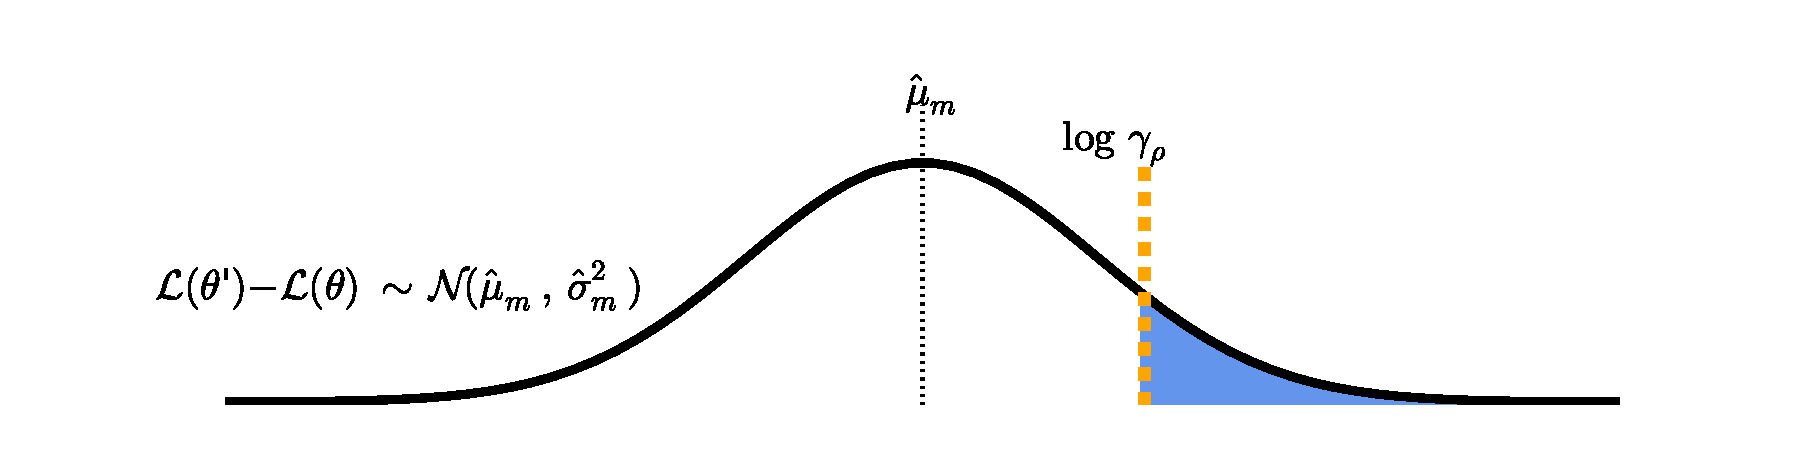
\includegraphics[width=\textwidth]{figs/accept.pdf}
\end{center}
\vspace{-0.2in}
\caption{We use a normal model for the difference of log posteriors at states~$\theta'$ 
and~$\theta$ as~${\mcL(\theta') - \mcL(\theta)} \sim \N(\hat{\mu}_m, \hat{\sigma}_m^2)$.
Thus, the predictor~$\PredEst{\rho}{m}$ is equal to the area under~$\N(\mu, \sigma^2)$
to the right of~$\log \gamma_\rho$.
Recall that~$\gamma_\rho$ is the precomputed random MH threshold of
Equation~\ref{eqn:precomputed-threshold} and depends on a
uniform random variate~${u \sim \Unif(0, 1)}$.
}
\label{fig:accept}
\end{figure}
%
\noi As illustrated in Figure~\ref{fig:accept}, we can now form the
predictor~$\PredEst{\rho}{m}$ by considering the tail probability
for~$\log \gamma_\rho$, where recall~$\gamma_\rho$ is defined in
Equation~\ref{eqn:precomputed-threshold}:
\begin{align}
\PredEst{\rho}{m} &= \int^\infty_{\log \gamma_\rho}
\N(z\given \hat{\mu}_m, \hat{\sigma}_m^2)\,\mathrm{d}z\\
&= 1 - \int_{-\infty}^{\log \gamma_\rho} \N(z\given \hat{\mu}_m, \hat{\sigma}_m^2)\,\mathrm{d}z \nn \\
&=\frac{1}{2} \left[
1 - \erf\left( \frac{\log \gamma_\rho - \log\hat{\mu}_m}{\sqrt{2}\hat{\sigma}_m}\right)
\right] \nn \\
&= \frac{1}{2}\left[
1 + \erf\left( \frac{\log\hat{\mu}_m - \log \gamma_\rho}{\sqrt{2}\hat{\sigma}_m}\right)
\right]\,.
\label{eqn:subset}
\end{align}

\end{document}



\section{Speedup with instantaneous, imperfect predictions}

%\subsection{Lower bound with an infinitely fast estimator}
%\subsection{Upper bound with an infinitely fast estimator}

If we could make instantaneous, perfect predictions, then predictive prefetching
would achieve perfect speedup, in an ideal system with zero communication costs
or other overheads.
In reality, we have access only to imperfect predictions, and we use
probabilistic models to characterize our uncertainty about these predictions.
In this section, we analyze the expected speedup of predictive prefetching,
as a function of predictor accuracy, for infinitely fast predictions in
an ideal system.

\begin{figure}[t!]
  \centering%
  \resizebox{\columnwidth}{!}{%
    \def\radius {9mm}
    \tikzstyle{empty}=[circle, thick, minimum size=\radius, font=\footnotesize]
    \tikzstyle{state}=[circle, thick, minimum size=\radius, font=\footnotesize, draw]
    \tikzstyle{compute}=[circle, thick, fill=CornflowerBlue, inner sep=0pt, minimum size=\radius, font=\footnotesize, draw]
    \begin{tikzpicture}[->,>=stealth',level/.style={sibling distance = 7cm/#1, level distance = 1.5cm}]
      \draw [white,-] (-6cm,-0.75cm) -- (6cm,-0.75cm);
   %   \draw [white,-] (-6cm,-2.25cm) -- (6cm,-2.25cm);
   %   \draw [white,-] (-6cm,-3.75cm) -- (6cm,-3.75cm);
      \node [state] (root) {}
      child{ node [state] {1} 
        child{ node [state] {$p$}
          child{ node [state] {$p^2$}
          edge from parent node[left] {$p$} }
          child{ node [state] {$pq$}
          edge from parent node[right] {$q$} }
          edge from parent node[left] {$p$} 
        }
        child{ node [state] {$q$}
          child{ node [state] {$qp$}
          edge from parent node[left] {$p$} }
          child{ node [state] {$q^2$}
          edge from parent node[right] {$q$} }
          edge from parent node[right] {$q$}
        }
        edge from parent node[left] {1} 
      }
      ;
      \node [empty] at (5.5cm, 0) {0};
      \node [empty] at (5.5cm, -1.5) {1};
      \node [empty] at (5.5cm, -3) {2};
      \node [empty] at (5.5cm, -4.5) {3};
      \draw [->, ultra thick, Dandelion] (root) to (root-1);
      \draw [->, ultra thick, Dandelion] (root-1) to (root-1-1);
      \draw [->, ultra thick, Dandelion] (root-1-1) to (root-1-1-1);
    \end{tikzpicture}
  }
  \caption{Metropolis--Hastings jobtree in our biased coin model.
  Nodes are arranged so that the left-most branch is the (unknown)
  true computation path (thick arrows). Furthermore, given a node,
  the predictor expects the left (right) child to be next on the path
  with probability~$p$~$(q)$, where~$p \ge q$ and~$p+q = 1$. 
  Each node is labeled by the probability the predictor expects it
  to be on the true path.
  The root is complete; workers are scheduled to the remaining nodes greedily.
  We index depth in the tree from~$0$ at the root.  
}
  \label{fig:biased-coin}
\end{figure}

Consider a specific MH simulation of fixed length.
Suppose we have access to a predictor~$\Predictor{\rho}$ that models the
conditional probability that~$x_\rho$ is accepted, given that~$\rho$ is on the 
computation path, as introduced in Section~\ref{sec:predictive-prefetching}.
%
We model the predictor's accuracy by a biased coin, depicted in
Figure~\ref{fig:biased-coin}.
Let~$p$ be the probability that the expected outcome is the true outcome
and let~${q = 1-p}$ be the corresponding probability that it is not.
We can think of~$p$ and~$q$ as the accuracy and error, respectively,
of the predictor.
%
Let~$\tau_J$ denote the MH simulation running time, using predictive prefetching 
with~$J$ workers. 
Then,~${S_J = \tau_1 / \tau_J}$ is the speedup relative to a single worker.
Our objective is to understand~$S_J$ as a function of~$q$ and~$J$.

In the limit of perfect predictions,~${q = 0}$ and predictive prefetching
obtains perfect, linear speedup, with~${S_J = J}$.
In the limit of uninformative predictions,~${q = 1/2}$ and predictive
prefetching reduces to the na\"ive scheme, leading to logarithmic speedup.
The expected speedup is~$\log_2 (J+1)$,
\eg ${\E[S_1] = 1}$, ${\E[S_3] = 2}$, ${\E[S_7] = 3}$.
Below, we analyze the expected speedup for imperfect predictions,
where~${0 < q < 1/2}$.
We do not study the adversarial scenario of malicious predictions,
where~${q > 1/2}$, which happens when we believe our predictors to be
informative, but they are actually incorrect on average.

To calculate expected speedup, we need to understand how the greedy scheme,
described in Section~\ref{sec:predictive-prefetching}, schedules workers on the jobtree.
For simplicity, we consider one `round'~\todo{Use BSP model?} of the algorithm, initialized as follows:
the jobtree is known to depth~$J$, where the root is considered depth~$0$,
the target has been evaluated at the root and nowhere else;
at all other nodes, only the predictor has been evaluated.
We break down our analysis into two parts.
First, we consider the scheduled workers' depth,
which gives us a lower bound on the expected speedup.
Then, we give a complete description of the workers' allocation,
which allows us to calculate the expected speedup.
Finally, we consider a scheme that combines predictive prefetching with
parallel computation at each node.


\subsection{Worker depth and simple bounds on speedup}
\label{sec:bounds}

In the limit of perfect predictions,~${q = 0}$, and predictive prefetching
schedules workers along the true computation path in the jobtree.
When~${0 < q < 1/2}$, our biased coin model assigns the~$k$-th node along the
true path a probability of~$p^k$, where the root is indexed by~${k = 0}$. 
In Figure~\ref{fig:biased-coin}, this corresponds to the left-most branch.
As long as~${p^k > pq}$, a greedy scheduling algorithm places at least~$k$
cores along this path before starting to consider alternate paths.
Let~$K$ denote the maximum value of~$k$ before the greedy algorithm starts 
to allocate cores away from a single path, \ie $K$ is the largest value of~$k$
satisfying~${p^k = (1-q)^k \ge q}$.  Then,
\be
K = \biggl\lfloor \frac{\log q }{\log(1-q)}\biggr\rfloor.
\label{eq:K}
\ee
For example, when~${q=0.1, 0.01, 0.001}$, then~${K=21, 458, 6904}$, respectively.
Figure~\ref{fig:speedup-K-q} plots~$K$ as a function of~$q$ on a log-log scale.
With~$K$ cores, the expected speedup is the sum of the 
probabilities of these nodes, giving us the following lower bound:
\[
\E[S_K] \ge \sum_{k=1}^K p^k = -1 + \sum_{k=0}^K p^k = -1 + \frac{1-p^{K+1}}{1-p}
= \frac{p-p^{K+1}}{1-p}
= \frac{(1-q) - (1-q)^{K+1}}{q}.
\]
Since~$K$ tells us about the depth of the tree, it also gives us an
upper bound on~$S_J$.
With~${J \le K}$ cores, they are all placed along the left branch, thus~${S_J < J}$.
With~${J > K}$ cores, for reasonable values of~$J$ and~$q$, workers are
allocated to other nodes at depths no greater than~$K$, thus~${S_J < K}$.
%Finally, with~${J > 2^K}$ cores, ${S_J < K + \log_2(J-K)}$.
Figure~\ref{fig:expected-speedup} depicts these lower and upper bounds
on the expected speedup, as a function of~$J$, for different values of~$q$.

\begin{figure}[t!]
\centering
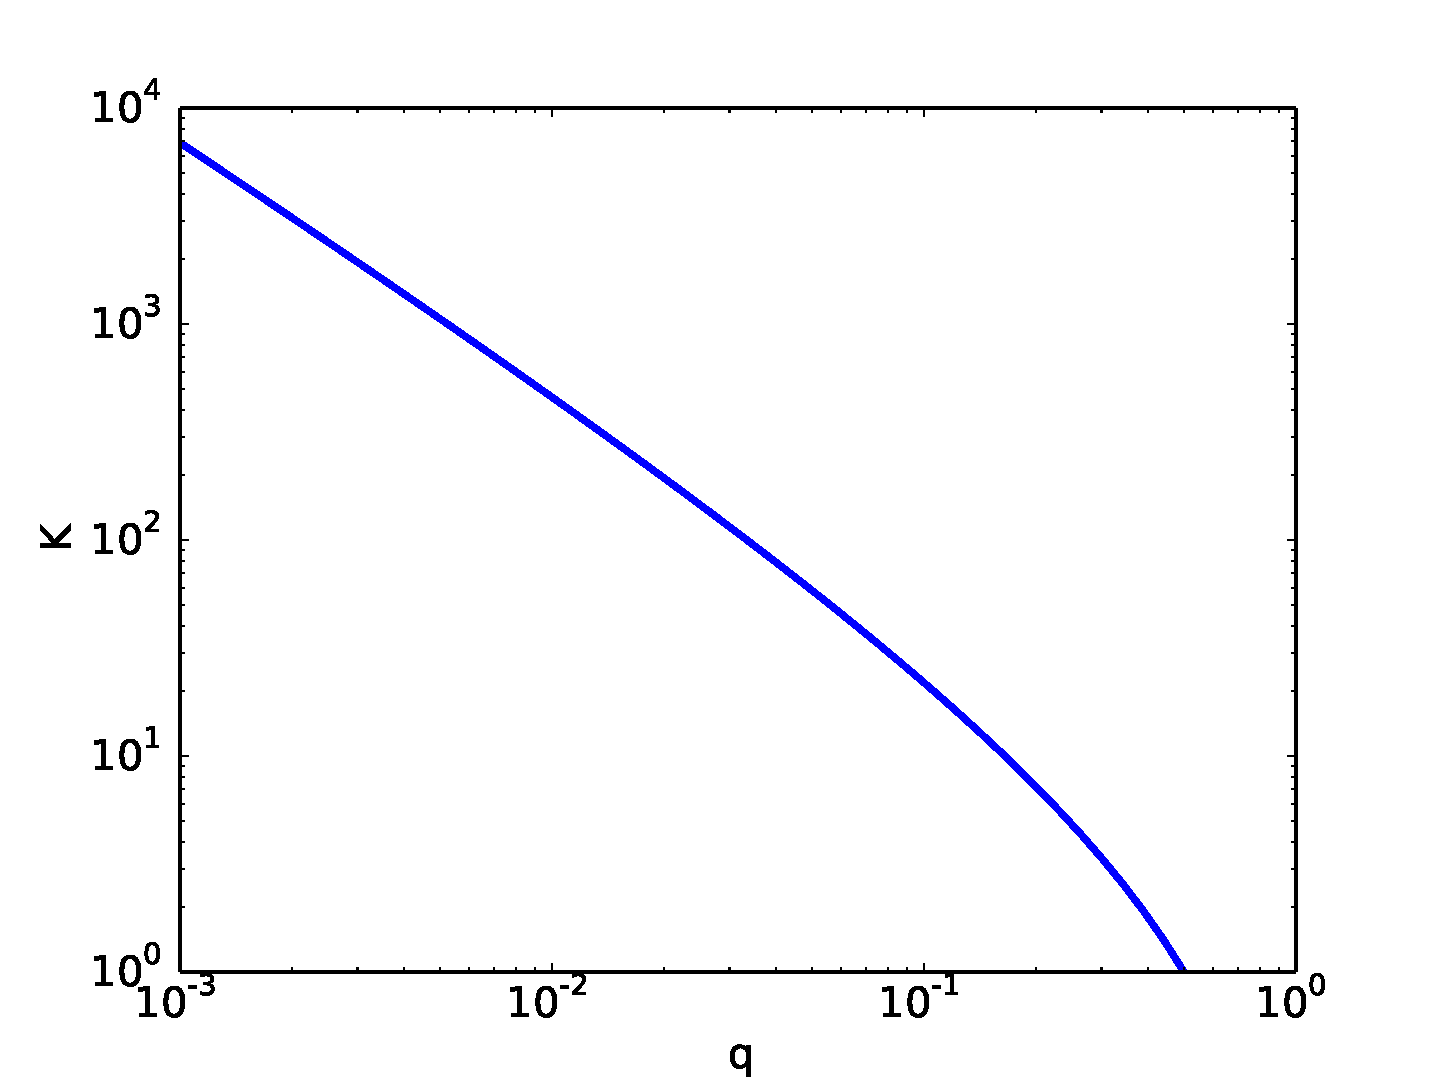
\includegraphics[width=0.65\textwidth]{figs/speedup-K-q.pdf}
\caption{$K$ as a function of~$q$, shown on a log-log plot.
${K = \log q  / \log(1-q)}$ is the maximum number of nodes allocated before the
greedy scheduling algorithm starts to place cores away from the single true path,
and~${0 < q < 1/2}$ is the error rate in our biased coin model.
}
\label{fig:speedup-K-q}
\end{figure}

\begin{figure}[t!]
\centering
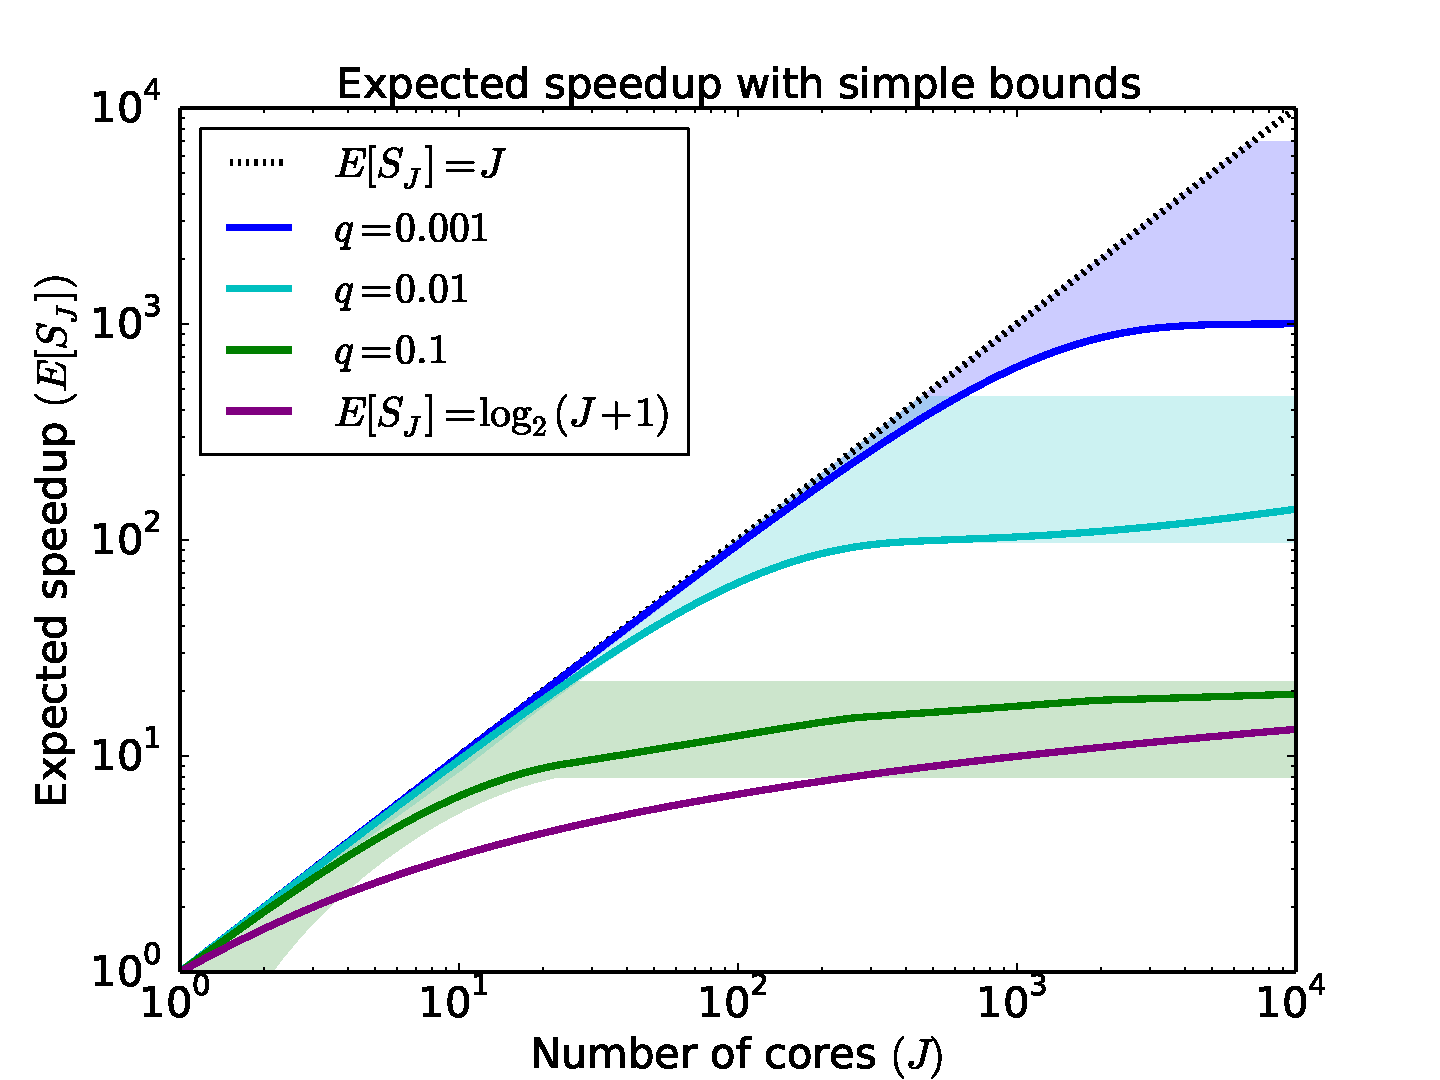
\includegraphics[width=0.65\textwidth]{figs/expected-speedup.pdf}
\caption{Expected speedup as a function of the number of workers.
The extremes of the shaded regions are the lower and upper bounds
for speedup from Section~\ref{sec:bounds}.
The solid lines show the sum of the~$J$ largest terms in~$U$, as described in
Section~\ref{sec:allocation}.
Different colors indicate different values of~$q$.
The dotted black line corresponds to perfect linear speedup;
the solid purple line corresponds to the na\"ive scheme, \ie ${q=0.5}$.
When~${q=0.1, 0.01, 0.001}$, then~${K=21, 458, 6904}$, respectively;
these values correspond to the (horizontal) upper bounds where~${J \ge K}$.
}
\label{fig:expected-speedup}
\end{figure}


\subsection{Worker allocation and expected speedup}
\label{sec:allocation}

The greedy algorithm places~$J$ cores at the~$J$ nodes with the
highest probabilities of occurring on the true path.  
Let us encode a node at depth~$i$ by a bit string 
${\gamma \in \{0, 1\}^i}$, where the root is at depth~0.
In our encoding introduced in Section~\ref{sec:bit-strings},
\bits{1}~(\bits{0}) denotes that, given a state~$\theta$,
the proposal~$\theta'$ is accepted~(rejected).
Here, let \bits{1}~(\bits{0}) denote that a prediction based on the
expected outcome is correct (incorrect) with probability ${p~(q = 1-p)}$. 

Let~${\Pr(\gamma \given q)}$ denote the probability that the node encoded by
bit string~$\gamma$ is on the true path, given~$q$, the probability that the
expected outcome from one node to the next is incorrect.
Let~$a$ and~$b$ be the number of~\bits{1}'s and~\bits{0}'s, respectively.
Then,
\[
p(\gamma \given q) = p^a q^b.
\]
The resulting expected speedup is the sum of the~$J$ largest terms in
\[
U = \{\Pr(\bits{0}), \Pr(\bits{1}), 
\Pr(\bits{00}), \Pr(\bits{01}), \Pr(\bits{10}), \Pr(\bits{11}), \dots\},
\]
where we have suppressed the dependency on~$q$ in our notation.
Figure~\ref{fig:expected-speedup} plots the expected~$S_J$ as a function of~$J$,
for different values of~$q$; it falls within the bounds mentioned previously.
To compute this sum, it is not necessary to exhaustively enumerate all the terms
up to depth~$J$; our above reasoning tells us that depth~$K$ suffices.
Let~$z$ be the number of~\bits{0}'s, \ie errors. 
We consider all terms up to depth~$K$, for~${z=0, \dots, 87}$:
%
\begin{itemize}
\item $z=0: \Pr(\bits{1}), \Pr(\bits{11}), \Pr(\bits{111}), \dots$
\item $z=1: \Pr(\bits{0}), \Pr(\bits{01}), \Pr(\bits{10}), 
	\Pr(\bits{011}), \Pr(\bits{101}), \Pr(\bits{110}), \dots$
\item $z=2: \Pr(\bits{00}), \Pr(\bits{001}), \Pr(\bits{010}), \Pr(\bits{100}), \dots$
\item $\dots$
\end{itemize}
%
We do not actually enumerate all of the above terms, but instead count
the number of terms in each group having the same probability,
\ie all terms for a particular~$z$ at the same depth in the tree.
For example, there are~3 bit strings of length~3 with~${z=1}$;
they all have probability~$p^2q$.

\subsection{Speculation plus parallelism at each node}
\label{sec:multi-way}

Finally, we consider the case where we combine parallel predictive prefetching
with parallelism at each node in the jobtree.
Figure~\ref{fig:multi-way} plots the expected speedup as a function of~$J$,
for 8-way and 64-way parallelism at each node.
Such a scheme would allow us to place more workers at higher-probability nodes,
and therefore achieve greater speedup.
As we noted in Section~\ref{sec:mcmc-prefetching},
\citet{strid-2010-prefetching} has experimented with this idea.

\begin{figure}[t!]
\centering
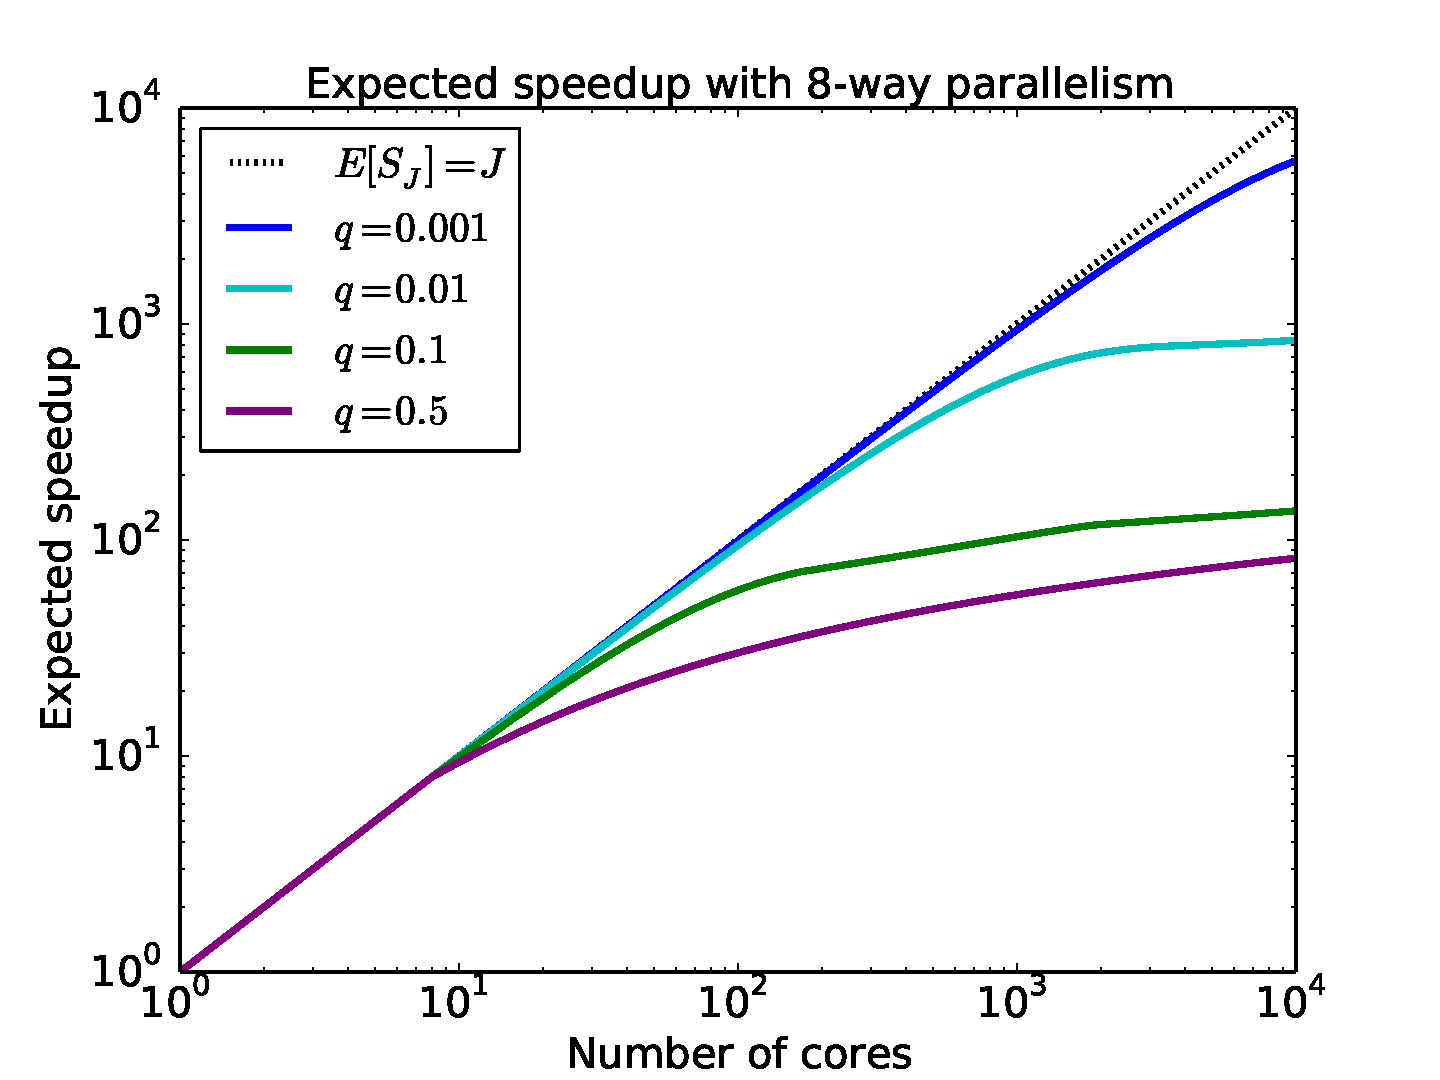
\includegraphics[width=0.65\textwidth]{figs/speedup-8.pdf}
\vskip2\baselineskip
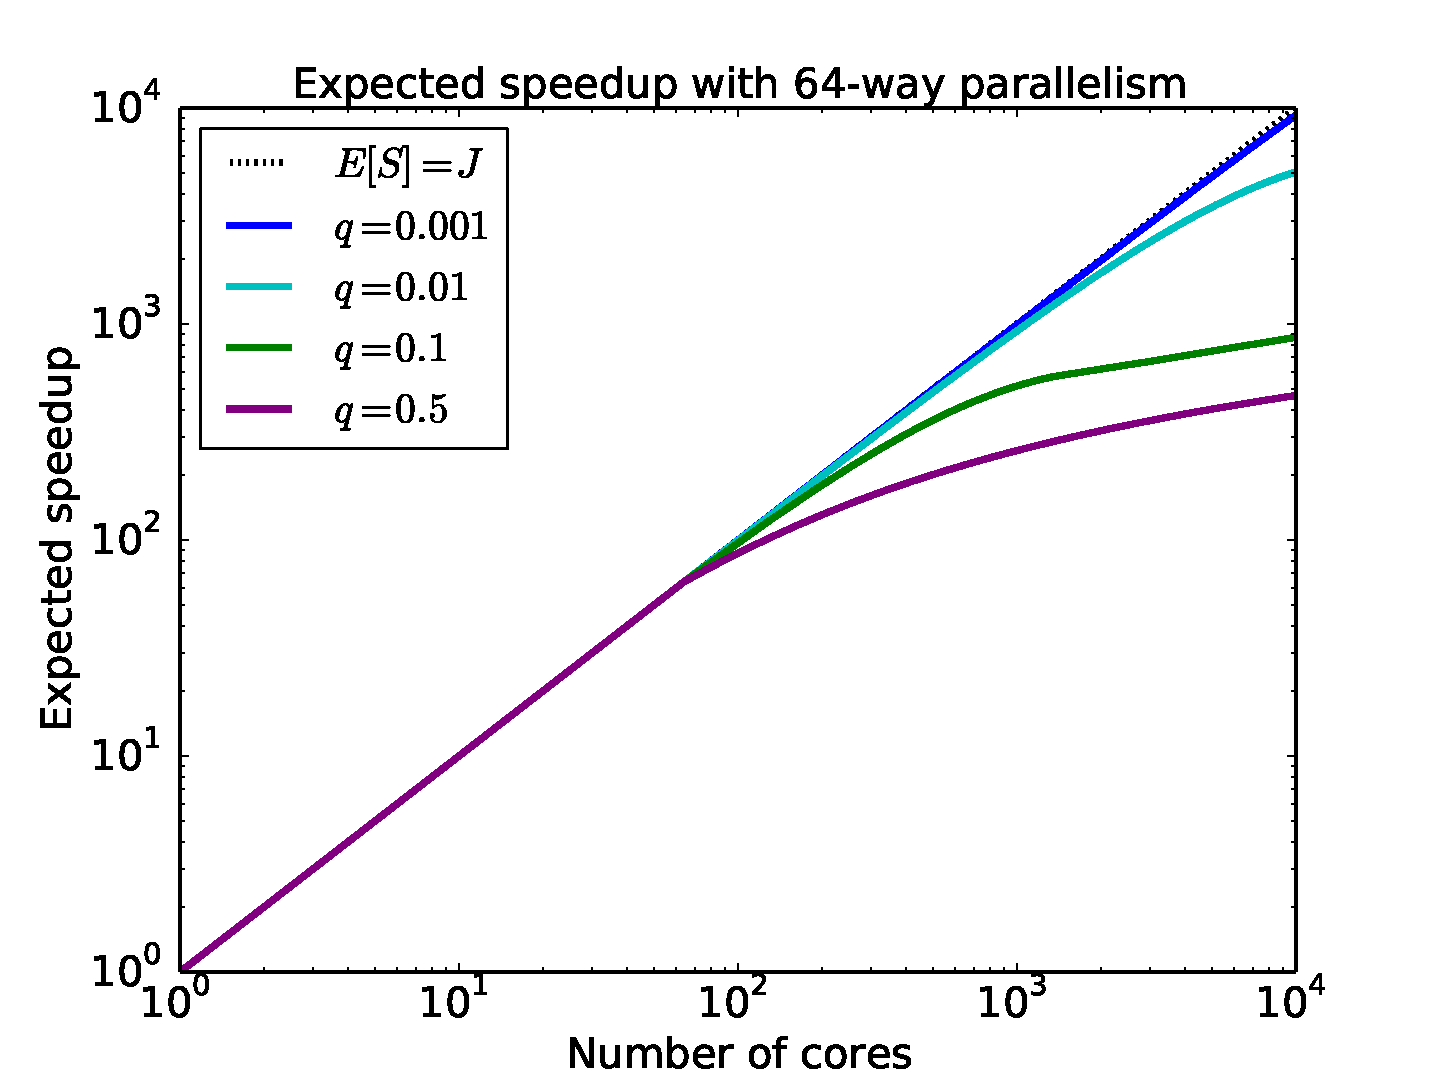
\includegraphics[width=0.65\textwidth]{figs/speedup-64.pdf}
\caption{Expected speedup as a function of~$J$,
with 8-way (top) and 64-way (bottom) parallelism at each node.
The dotted black line corresponds to perfect linear speedup;
the solid purple line $(q=0.5)$ corresponds to the na\"ive scheme with
parallelism at each node.}
\label{fig:multi-way}
\end{figure}

\end{document}